\RequirePackage{atbegshi}
\documentclass[compress,aspectratio=169]{beamer}\usepackage[]{graphicx}\usepackage[dvipsnames]{xcolor}
% maxwidth is the original width if it is less than linewidth
% otherwise use linewidth (to make sure the graphics do not exceed the margin)
\makeatletter
\def\maxwidth{ %
  \ifdim\Gin@nat@width>\linewidth
    \linewidth
  \else
    \Gin@nat@width
  \fi
}
\makeatother

\definecolor{fgcolor}{rgb}{0.345, 0.345, 0.345}
\newcommand{\hlnum}[1]{\textcolor[rgb]{0.686,0.059,0.569}{#1}}%
\newcommand{\hlsng}[1]{\textcolor[rgb]{0.192,0.494,0.8}{#1}}%
\newcommand{\hlcom}[1]{\textcolor[rgb]{0.678,0.584,0.686}{\textit{#1}}}%
\newcommand{\hlopt}[1]{\textcolor[rgb]{0,0,0}{#1}}%
\newcommand{\hldef}[1]{\textcolor[rgb]{0.345,0.345,0.345}{#1}}%
\newcommand{\hlkwa}[1]{\textcolor[rgb]{0.161,0.373,0.58}{\textbf{#1}}}%
\newcommand{\hlkwb}[1]{\textcolor[rgb]{0.69,0.353,0.396}{#1}}%
\newcommand{\hlkwc}[1]{\textcolor[rgb]{0.333,0.667,0.333}{#1}}%
\newcommand{\hlkwd}[1]{\textcolor[rgb]{0.737,0.353,0.396}{\textbf{#1}}}%
\let\hlipl\hlkwb

\usepackage{framed}
\makeatletter
\newenvironment{kframe}{%
 \def\at@end@of@kframe{}%
 \ifinner\ifhmode%
  \def\at@end@of@kframe{\end{minipage}}%
  \begin{minipage}{\columnwidth}%
 \fi\fi%
 \def\FrameCommand##1{\hskip\@totalleftmargin \hskip-\fboxsep
 \colorbox{shadecolor}{##1}\hskip-\fboxsep
     % There is no \\@totalrightmargin, so:
     \hskip-\linewidth \hskip-\@totalleftmargin \hskip\columnwidth}%
 \MakeFramed {\advance\hsize-\width
   \@totalleftmargin\z@ \linewidth\hsize
   \@setminipage}}%
 {\par\unskip\endMakeFramed%
 \at@end@of@kframe}
\makeatother

\definecolor{shadecolor}{rgb}{.97, .97, .97}
\definecolor{messagecolor}{rgb}{0, 0, 0}
\definecolor{warningcolor}{rgb}{1, 0, 1}
\definecolor{errorcolor}{rgb}{1, 0, 0}
\newenvironment{knitrout}{}{} % an empty environment to be redefined in TeX

\usepackage{alltt}

% % % % % % % % % % % % % % %
%             MY PACKAGES 
% % % % % % % % % % % % % % %
\usepackage{graphicx}
\usepackage{dcolumn}
\usepackage[export]{adjustbox}
\usepackage[dvipsnames]{xcolor}
\usepackage{amssymb,amsmath}
\usepackage{threeparttable}

\usepackage{pgfplots}
\pgfplotsset{compat=1.11}
\usepgfplotslibrary{fillbetween}

\usepackage{rotating}
\usepackage{import}
\usepackage{array}
\usepackage{tabularx}
\usepackage{float}
\usepackage{pifont}
\usepackage{hyperref}
\usepackage{multirow}

\usepackage{tikz}
\usetikzlibrary{arrows,decorations.pathreplacing,positioning}

\usepackage{listings}
\usepackage{color}
\definecolor{dkgreen}{rgb}{0,0.6,0}
\definecolor{gray}{rgb}{0.5,0.5,0.5}
\definecolor{mauve}{rgb}{0.58,0,0.82}
\lstset{
  language=R,
  basicstyle=\TINY,
  numbers=left,
  numberstyle=\tiny\color{gray},
  stepnumber=1,
  numbersep=5pt,
  backgroundcolor=\color{white},
  showspaces=false,
  showstringspaces=false,
  showtabs=false,
  frame=single,
  rulecolor=\color{black},
  tabsize=1,
  captionpos=b,
  breaklines=true,
  breakatwhitespace=false,
  title=\lstname,
  keywordstyle=\color{blue},
  commentstyle=\color{dkgreen},
  stringstyle=\color{mauve},
  escapeinside={\%*}{*)},
  morekeywords={*,...}
}

% % % % % % % % % % % % % % %
%           PACKAGE CUSTOMIZATION
% % % % % % % % % % % % % % %

\usepackage[math]{iwona}
\usetheme{Singapore}
\usecolortheme{rose}
\makeatletter
\beamer@theme@subsectiontrue
\makeatother

% navigation dots behavior
\makeatletter
\def\slideentry#1#2#3#4#5#6{%
  \ifnum#6=\c@part\ifnum#2>0\ifnum#3>0%
    \ifbeamer@compress%
      \advance\beamer@xpos by1\relax%
    \else%
      \beamer@xpos=#3\relax%
      \beamer@ypos=#2\relax%
    \fi%
  \hbox to 0pt{%
    \beamer@tempdim=-\beamer@vboxoffset%
    \advance\beamer@tempdim by-\beamer@boxsize%
    \multiply\beamer@tempdim by\beamer@ypos%
    \advance\beamer@tempdim by -.05cm%
    \raise\beamer@tempdim\hbox{%
      \beamer@tempdim=\beamer@boxsize%
      \multiply\beamer@tempdim by\beamer@xpos%
      \advance\beamer@tempdim by -\beamer@boxsize%
      \advance\beamer@tempdim by 1pt%
      \kern\beamer@tempdim
      \global\beamer@section@min@dim\beamer@tempdim
      \hbox{\beamer@link(#4){%
          \usebeamerfont{mini frame}%
          \ifnum\c@section>#1%
            \usebeamercolor{mini frame}%
            \usebeamertemplate{mini frame in other subsection}%
          \else%
            \ifnum\c@section=#1%
              \ifnum\c@subsection>#2%
                \usebeamercolor[fg]{mini frame}%
                \usebeamertemplate{mini frame}%
              \else%
                \ifnum\c@subsection=#2%
                  \usebeamercolor[fg]{mini frame}%
                  \ifnum\c@subsectionslide<#3%
                    \usebeamertemplate{mini frame in current subsection}%
                  \else%
                    \usebeamertemplate{mini frame}%
                  \fi%
                \else%
                  \usebeamercolor{mini frame}%
                  \usebeamertemplate{mini frame in other subsection}%
                \fi%
              \fi%
            \else%
              \usebeamercolor{mini frame}%
              \usebeamertemplate{mini frame in other subsection}%
            \fi%
          \fi%
        }}}\hskip-10cm plus 1fil%
  }\fi\fi%
  \else%
  \fakeslideentry{#1}{#2}{#3}{#4}{#5}{#6}%
  \fi\ignorespaces
}
\makeatother

\beamertemplatenavigationsymbolsempty
\makeatletter
\setbeamertemplate{footline}{
\leavevmode%
\hbox{%
\begin{beamercolorbox}[wd=1\paperwidth,ht=2.25ex,dp=2ex,center]{title in head/foot}%
\usebeamerfont{title in head/foot}\insertshorttitle
\end{beamercolorbox}%
\begin{beamercolorbox}[wd=1\paperwidth,ht=2.25ex,dp=2ex,center]{date in head/foot}%
\end{beamercolorbox}}%
}
\makeatother

\makeatletter
\let\beamer@writeslidentry@miniframeson=\beamer@writeslidentry
\def\beamer@writeslidentry@miniframesoff{%
  \expandafter\beamer@ifempty\expandafter{\beamer@framestartpage}{}%
  {%
    \clearpage\beamer@notesactions%
  }
}
\newcommand*{\miniframeson}{\let\beamer@writeslidentry=\beamer@writeslidentry@miniframeson}
\newcommand*{\miniframesoff}{\let\beamer@writeslidentry=\beamer@writeslidentry@miniframesoff}
\makeatother

\newcommand<>{\fullsizegraphic}[1]{
  \begin{textblock*}{0cm}(-1cm,-3.78cm)
  \includegraphics[width=\paperwidth]{#1}
  \end{textblock*}
}

\hypersetup{colorlinks,urlcolor=[rgb]{0.01,0.28,1.0},linkcolor=[rgb]{0.01,0.28,1.0}}

% % % % % % % % % % % % % % %
%           DOCUMENT ID
% % % % % % % % % % % % % % %

\title{\input{title.txt}\unskip}
\author[shortname]{Hector Bahamonde \inst{1} \and Andrea Canales \inst{2}}
\institute[shortinst]{\inst{1} University of Turku, Finland \and \inst{2} O$'$Higgins University, Chile}
\date{10 minute talk}
\IfFileExists{upquote.sty}{\usepackage{upquote}}{}
\begin{document}





%====================
% TITLE SLIDE
%====================

\begin{frame}
\titlepage
\end{frame}

%====================
% INTRODUCTION
%====================

\section{Introduction}
\subsection{A sequencing story}

\begin{frame}[c]{Why sequencing matters}
\begin{itemize}
  \item Think of two familiar situations:
  \begin{itemize}
    \item A buyer walks up to you on the street: ``I will give you 50 euros for that concert ticket.''
    \item You post the same ticket online and say: ``I will sell it for 80 euros; take it or leave it.''
  \end{itemize}
  \item Same good, same buyer, same seller, same environment.
  \item But who moves first changes:
  \begin{itemize}
    \item Who has bargaining power.
    \item Who gets more surplus.
    \item Which transactions actually happen.
  \end{itemize}
  \item In clientelism, we almost always assume \textbf{parties move first} (vote buying).
  \item This paper asks: \textbf{what happens when voters move first and sell?}
\end{itemize}
\end{frame}

\subsection{The neglected vote seller}

\begin{frame}[c]{Clientelism research has a lopsided market view}
\begin{itemize}
  \item Classic view: clientelism as \textbf{party-initiated demand} for votes.
  \begin{itemize}
    \item Who do parties buy from? Core vs swing?
    \item Do they buy more when elections are close or safe?
  \end{itemize}
  \item But real clientelist exchanges are \textbf{reciprocal}:
  \begin{itemize}
    \item Ethnographers show voters, neighborhood leaders, and brokers often initiate exchanges.
    \item Many relationships are explicitly described as \textbf{client-initiated}.
  \end{itemize}
  \item Yet quantitative work:
  \begin{itemize}
    \item Heavily focused on vote buying.
    \item Almost no systematic modeling of \textbf{vote sellers} and their strategies.
  \end{itemize}
  \item We argue: to understand clientelism, we must put \textbf{voters as strategic sellers} on equal footing with parties.
\end{itemize}
\end{frame}

\begin{frame}[c]{The imbalance in the literature}
\centering
\includegraphics[width=0.75\textwidth]{/Users/hectorbahamonde/research/Exp_Vote_Selling/histogram_meta_plot.png}
\vspace{0.2cm}

{\small Annual frequency of Web of Science publications whose abstracts include the terms ``vote buying'' and ``vote selling''.}
\end{frame}

\subsection{This paper}

\begin{frame}[c]{What we do}
\begin{itemize}
  \item Conceptual move:
  \begin{itemize}
    \item Treat \textbf{vote buying} and \textbf{vote selling} as two institutional variants of the same market.
    \item The key institutional rule is \textbf{who moves first}.
  \end{itemize}
  \item Theory:
  \begin{itemize}
    \item Simple spatial model with one voter and two parties.
    \item Institutional variant 1: \textbf{party-initiated vote buying}.
    \item Institutional variant 2: \textbf{voter-initiated vote selling}.
  \end{itemize}
  \item Experiment:
  \begin{itemize}
    \item Laboratory game that mirrors the model.
    \item Same ideology, budgets, and electoral stakes; only sequencing changes.
  \end{itemize}
  \item Focus today:
  \begin{itemize}
    \item Intuition and key notation from the model.
    \item Experimental design and empirical results.
    \item What we learn about \textbf{who benefits} from clientelism when voters sell.
  \end{itemize}
\end{itemize}
\end{frame}

%====================
% THEORY
%====================

\section{Theory}
\subsection{Sequencing as an institution}

\begin{frame}[c]{Two institutional variants of the same exchange}
\centering
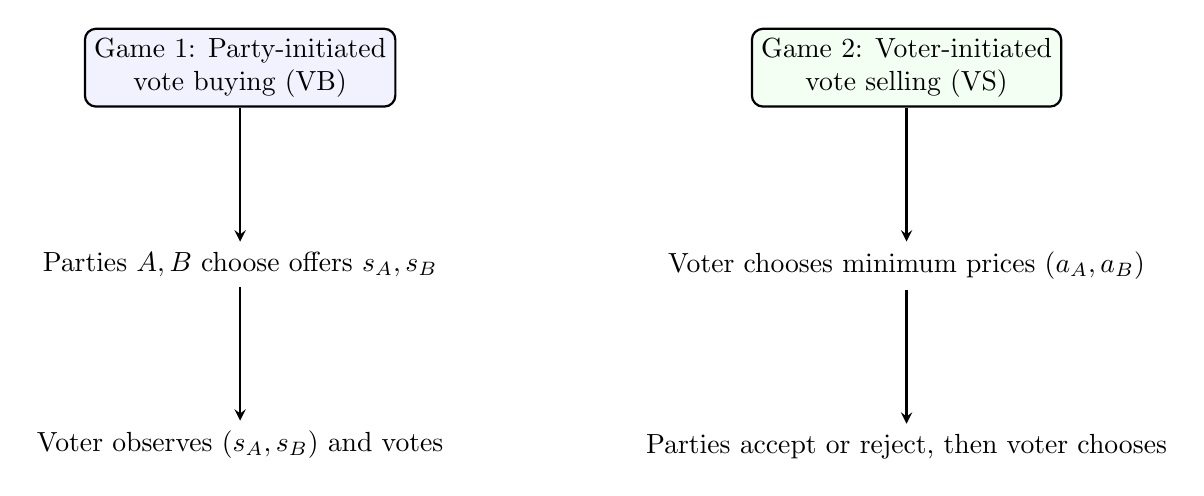
\begin{tikzpicture}[node distance=1.7cm,>=stealth,thick]
\node (vb) [rectangle,draw,rounded corners,align=center,fill=blue!5] {Game 1: Party-initiated \\ vote buying (VB)};
\node (vs) [rectangle,draw,rounded corners,align=center,fill=green!5,right=4.5cm of vb] {Game 2: Voter-initiated \\ vote selling (VS)};

\node (vb1) [below=of vb] {Parties $A,B$ choose offers $s_A,s_B$};
\node (vb2) [below=of vb1] {Voter observes $(s_A,s_B)$ and votes};

\node (vs1) [below=of vs] {Voter chooses minimum prices $(a_A,a_B)$};
\node (vs2) [below=of vs1] {Parties accept or reject, then voter chooses};

\draw[->] (vb) -- (vb1);
\draw[->] (vb1) -- (vb2);
\draw[->] (vs) -- (vs1);
\draw[->] (vs1) -- (vs2);
\end{tikzpicture}

\vspace{0.4cm}
\begin{itemize}
  \item \textbf{Same}: one pivotal voter, two parties, payoffs, budgets, electoral stakes.
  \item \textbf{Different}: only \textbf{who moves first} and hence who has bargaining power.
\end{itemize}
\end{frame}

\subsection{Key notation (light version)}

\begin{frame}[c]{Players, preferences, and stakes}
\begin{itemize}
  \item Two parties $i \in \{A,B\}$ and one pivotal voter $j$.
  \item One-dimensional policy space: $\gamma \in \{1,\dots,100\}$ with $\gamma_A < \gamma_B$.
  \item Voter has ideal point $x_j$; ideological utility if party $i$ wins:
  \[
  u_j(\gamma_i) = D - \lvert x_j - \gamma_i \rvert,
  \]
  where $D$ keeps payoffs positive.
  \item Voter prefers party
  \[
    i^\ast = \arg\max_{i \in \{A,B\}} u_j(\gamma_i).
  \]
  \item Ideological advantage of the core party:
  \[
    \Delta = u_j(\gamma_{i^\ast}) - u_j(\gamma_{-i^\ast}) > 0.
  \]
  This is the \textbf{minimum compensating transfer} needed to flip the vote.
\end{itemize}
\end{frame}

\begin{frame}[c]{Electoral risk and transfers}
\begin{itemize}
  \item Voter is pivotal with probability $\pi>0$.
  \item Party $i$ values winning at $W_i$, so its electoral stake is
  \[
    R_i = \pi W_i.
  \]
  \item Think of $R_i$ as how much the party is willing to pay for the pivotal vote.
  \item Transfers:
  \begin{itemize}
    \item Vote buying: parties offer $s_i \ge 0$.
    \item Vote selling: voter requests $a_i \ge 0$.
  \end{itemize}
  \item Voter total utility from voting for $i$ and receiving transfer $t_i$:
  \[
    U_j(i,t_i) = u_j(\gamma_i) + t_i.
  \]
\end{itemize}
\end{frame}

\subsection{Core logic of the model}

\begin{frame}[c]{Game 1: Party-initiated vote buying}
\begin{itemize}
  \item Parties observe ideology and stakes $(x_j,\gamma_A,\gamma_B,R_A,R_B)$.
  \item Each chooses offer $s_i$ simultaneously.
  \item Voter sees $(s_A,s_B)$ and chooses a party.
  \item In the symmetric benchmark with $R_A = R_B = R$ and $R > \Delta$:
  \[
    s_{i^\ast}^{VB} = \Delta, \quad s_{-i^\ast}^{VB} = 0.
  \]
  \item So:
  \begin{itemize}
    \item The ideologically preferred party $i^\ast$ buys the vote.
    \item The opponent does not buy.
    \item Transfers concentrate on \textbf{core} voters.
  \end{itemize}
  \item This recovers the familiar \textbf{core targeting} result when parties move first.
\end{itemize}
\end{frame}

\begin{frame}[c]{Game 2: Voter-initiated vote selling}
\begin{itemize}
  \item Voter proposes minimum acceptable prices $(a_A,a_B)$.
  \item Party $i$ accepts only if $a_i \le R_i$.
  \item Let $W$ be the \textbf{electorally stronger party} with $R_W > R_{-W}$.
  \item When $W$ is ideologically distant (not the core party):
  \[
    \text{Voter can set } a_W \approx R_W, \text{ and a lower } a_{i^\ast},
  \]
  so that both parties accept but the vote is sold to $W$.
  \item Intuition:
  \begin{itemize}
    \item Strong party has more at stake and a higher maximum willingness to pay.
    \item Voter exploits that stake to \textbf{sell to the opponent expected to win}.
  \end{itemize}
\end{itemize}
\end{frame}

\begin{frame}[c]{Hypotheses}
\begin{itemize}
  \item \textbf{H1 (Core targeting under party initiative):}
  \begin{itemize}
    \item When parties move first, transfers concentrate on ideologically close voters.
  \end{itemize}
  \item \textbf{H2 (Selling to the winning opponent):}
  \begin{itemize}
    \item When voters move first, they are more likely to sell to the party expected to win, even if that party is ideologically distant.
  \end{itemize}
  \item \textbf{H3 (Higher voter payoffs when parties initiate):}
  \begin{itemize}
    \item Because parties tend to overspend when they initiate vote buying, voters should earn higher expected payoffs in VB than in VS.
  \end{itemize}
\end{itemize}
\end{frame}

%====================
% EXPERIMENT
%====================

\section{Experimental design}
\subsection{Setup and roles}

\begin{frame}[c]{Laboratory implementation}
\begin{itemize}
  \item \textbf{Subjects and implementation}
  \begin{itemize}
    \item 102 adult participants in a Chilean lab, implemented in \texttt{oTree}.
    \item Show-up fee plus performance-based earnings in experimental points.
  \end{itemize}
  \item \textbf{Roles}
  \begin{itemize}
    \item Each game has three real players: Party A, Party B, Voter.
    \item Each subject plays three independent games; full re-randomization each time.
  \end{itemize}
  \item \textbf{Information}
  \begin{itemize}
    \item Ideological payoffs for the voter under A and B.
    \item Party budgets (identical within a game).
    \item Fictional vote shares determining whether the real voter is pivotal.
    \item All information is common knowledge.
  \end{itemize}
\end{itemize}
\end{frame}

\begin{frame}[c]{Experimental flow}
\centering
\includegraphics[width=\textwidth]{/Users/hectorbahamonde/research/Exp_Vote_Selling/experimental_flow.pdf}

\vspace{0.2cm}
\begin{itemize}
  \item Two variants implemented in identical environments:
  \begin{itemize}
    \item Game 1: parties offer, voter chooses.
    \item Game 2: voter requests, parties accept or reject, voter chooses.
  \end{itemize}
\end{itemize}
\end{frame}

\subsection{Ideology and electoral risk}

\begin{frame}[c]{Ideology, budgets, and pivotality}
\begin{itemize}
  \item \textbf{Ideological positions}
  \begin{itemize}
    \item For each game, the voter sees: points if A wins, points if B wins.
    \item This implements $u_j(\gamma_A)$ and $u_j(\gamma_B)$ and the ideological gap $\Delta$.
  \end{itemize}
  \item \textbf{Party budgets}
  \begin{itemize}
    \item Randomly drawn, identical for both parties in a given game.
    \item Constrain feasible offers or acceptable requested prices.
  \end{itemize}
  \item \textbf{Electoral risk}
  \begin{itemize}
    \item Fictional electorate with 3 or 5 additional voters.
    \item Vote shares assigned to A and B imply either a close or safe race.
    \item Real subject voter can be pivotal or not.
  \end{itemize}
\end{itemize}
\end{frame}

%====================
% EMPIRICAL RESULTS
%====================

\section{Empirical results}
\subsection{Behavior in the two games}

\begin{frame}[c]{Vote buying offers vs vote selling requests}
\centering
\includegraphics[width=\textwidth]{/Users/hectorbahamonde/research/Exp_Vote_Selling/depvarplot.png}
\vspace{0.2cm}

{\small Distributions of vote-buying offers (left) and vote-selling requests (right), as a share of parties budgets.}
\end{frame}

\begin{frame}[c]{What we learn from the distributions}
\begin{itemize}
  \item \textbf{Vote buying (VB):}
  \begin{itemize}
    \item Offers cluster at zero and at a small interior value that matches the compensating transfer $\Delta$.
    \item Behavior tracks the theoretical core-targeting equilibrium: core party buys, opponent often offers zero.
  \end{itemize}
  \item \textbf{Vote selling (VS):}
  \begin{itemize}
    \item Requested prices are widely dispersed.
    \item Many voters ask for very small transfers from at least one party.
    \item Many also ask for prices close to the party budget, especially from electorally strong parties.
  \end{itemize}
  \item This motivates modeling \textbf{requested prices} in VS as our main empirical window on seller behavior.
\end{itemize}
\end{frame}

\subsection{Pricing votes under vote selling}

\begin{frame}[c]{Modeling requested prices}
\begin{itemize}
  \item Unit of analysis: voter–party dyads in the vote-selling game.
  \item Dependent variable:
  \[
    Y_{di} = \frac{a_{di}}{B_{di}} \times 100,
  \]
  requested price as percentage of party $i$ budget.
  \item Key predictors:
  \begin{itemize}
    \item Ideological distance between voter and party.
    \item Party vote share in the fictional electorate (electoral strength).
    \item Interaction: ideology $\times$ vote share.
    \item Indicator for whether the real voter is pivotal.
  \end{itemize}
  \item Method:
  \begin{itemize}
    \item Linear model with clustered standard errors at the voter level.
  \end{itemize}
\end{itemize}
\end{frame}

\begin{frame}[c]{Selling to the electorally strong opponent}
\centering
\includegraphics[width=0.6\textwidth]{/Users/hectorbahamonde/research/Exp_Vote_Selling/m1plot.png}
\vspace{0.2cm}

{\small Predicted requested prices as a function of ideological distance and party electoral strength.}
\end{frame}

\begin{frame}[c]{Interpreting the pricing patterns}
\begin{itemize}
  \item For \textbf{electorally weak} parties:
  \begin{itemize}
    \item Requested prices \textbf{decrease} with ideological distance.
    \item When the weak party is close, voters ask for higher transfers to insure against its likely loss.
    \item When it is far, requested prices approach zero.
  \end{itemize}
  \item For \textbf{electorally strong} parties:
  \begin{itemize}
    \item Requested prices \textbf{increase} with ideological distance.
    \item When the strong party is distant, voters escalate demands up to its budget.
    \item Voters exploit the higher stake $R_i$ of strong parties.
  \end{itemize}
  \item This matches \textbf{H2}: when voters initiate, they strategically sell to the opponent expected to win and charge that party more.
\end{itemize}
\end{frame}

\subsection{Who gains from each institution?}

\begin{frame}[c]{Payoffs by role and by game}
\centering
\includegraphics[width=0.7\textwidth]{/Users/hectorbahamonde/research/Exp_Vote_Selling/payoffs_plot.png}
\vspace{0.2cm}

{\small Mean payoffs for voters and parties under vote buying (VB) and vote selling (VS) with non-parametric confidence intervals.}
\end{frame}

\begin{frame}[c]{Does initiative change who wins the game?}
\begin{itemize}
  \item \textbf{Parties:}
  \begin{itemize}
    \item Party payoffs are similar or slightly higher in VS relative to VB.
    \item Moving initiative to voters does not reduce parties utilities.
  \end{itemize}
  \item \textbf{Voters:}
  \begin{itemize}
    \item Voters earn systematically \textbf{higher payoffs} when parties move first (VB).
    \item In VS, high requested prices are often rejected; some voters end up with only ideological payoffs.
  \end{itemize}
  \item This matches \textbf{H3}: the house (parties) does at least as well or better when voters try to sell; voters actually do better when parties initiate the exchange.
\end{itemize}
\end{frame}

%====================
% DISCUSSION
%====================

\section{Discussion}
\subsection{What we learn}

\begin{frame}[c]{Main takeaways}
\begin{itemize}
  \item \textbf{Institutional rule}: who moves first matters for:
  \begin{itemize}
    \item Who is targeted (core vs strong opponent).
    \item How much is paid.
    \item How surplus is split between parties and voters.
  \end{itemize}
  \item When \textbf{parties initiate} (vote buying):
  \begin{itemize}
    \item Transfers concentrate on \textbf{core} voters.
    \item Parties often overspend under electoral risk.
    \item Voters capture a larger share of surplus.
  \end{itemize}
  \item When \textbf{voters initiate} (vote selling):
  \begin{itemize}
    \item Voters charge higher prices to electorally strong, ideologically distant parties.
    \item Many expensive demands are rejected, lowering average voter payoffs.
    \item Parties are at least as well off as in vote buying.
  \end{itemize}
\end{itemize}
\end{frame}

\subsection{Implications and limits}

\begin{frame}[c]{Implications and next steps}
\begin{itemize}
  \item Conceptually:
  \begin{itemize}
    \item Clientelism is best viewed as a \textbf{market} where both demand and supply matter.
    \item ``Vote buying'' and ``vote selling'' are two institutional faces of the same exchange.
  \end{itemize}
  \item Empirically:
  \begin{itemize}
    \item Initiative helps explain puzzles in core–swing targeting and surplus allocation.
    \item It is not enough to ask \emph{who parties buy}; we must also ask \emph{who voters can most profitably sell to}.
  \end{itemize}
  \item Limitations and extensions:
  \begin{itemize}
    \item One-shot lab game, no brokers, no repeated interactions or sanctions.
    \item Next steps: multi-voter and multi-party environments, networked brokers, field and survey experiments that vary who initiates.
  \end{itemize}
\end{itemize}
\end{frame}

%====================
% END
%====================

\miniframesoff
\begin{frame}[c]{Thank you}
\begin{center}
\vspace{-0.5cm}
\includegraphics[scale=0.05]{/Users/hectorbahamonde/research/Economic_Experiment_Vote_Selling/Resources_Presentation/qr-code.pdf}
\end{center}
\begin{itemize}
  \item Paper and abstract: {\color{blue}www.HectorBahamonde.com}
  \item Feedback very welcome.
\end{itemize}
\end{frame}

\end{document}
